\documentclass{article}
\usepackage{amsthm,authblk,fullpage,amssymb}

\usepackage[utf8]{inputenc}
\usepackage{tikz}
\usepackage{comment}
\usetikzlibrary{calc,decorations, decorations.pathreplacing,decorations.pathmorphing,arrows}
\usepackage{amssymb}
\usepackage{enumerate}
\usepackage{mathtools}

 \usepackage[hidelinks]{hyperref}
  \usepackage[capitalise]{cleveref}
\usepackage{breakurl}

 \theoremstyle{plain}
  \newtheorem{theorem}{Theorem}[section]
  \newtheorem{lemma}[theorem]{Lemma}  
  \newtheorem{observation}[theorem]{Observation}  
  \newtheorem{corollary}[theorem]{Corollary}  
  \newtheorem{fact}[theorem]{Fact}
  \crefname{figure}{Figure}{Figures}
  \theoremstyle{definition}
  \newtheorem{hypothesis}[theorem]{Hypothesis}
  \newtheorem{problem}[theorem]{Problem}
  \theoremstyle{remark}
  \newtheorem{remark}[theorem]{Remark}
  \newtheorem{example}[theorem]{Example}
  
\crefname{hypothesis}{Hypothesis}{Hypotheses} 


\renewcommand{\P}{\mathcal{P}}
\newcommand{\ww}{\mathbf{w}}
\newcommand{\pp}{\mathbf{p}}
\newcommand{\qq}{\mathbf{q}}
\newcommand{\QQ}{\mathbf{Q}}
\renewcommand{\SS}{\mathbf{S}}
\newcommand{\NN}{\mathbf{N}}
\newcommand{\SQ}{\mathit{SQ}}
\renewcommand{\Alph}{\mathrm{Alph}}
\newcommand{\Fib}{\mathit{Fib}}
\newcommand{\lleft}{\psi}
\newcommand{\eps}{\varepsilon}
\newcommand{\SQABEL}{\SQ_{\mathrm{Abel}}}
\newcommand{\SQPABEL}{\SQ'_{\mathrm{Abel}}}
\newcommand{\SQPARAM}{\SQ_{\mathrm{param}}}
\newcommand{\SQPPARAM}{\SQ'_{\mathrm{param}}}
\newcommand{\SQOP}{\SQ_{\mathrm{op}}}
\newcommand{\SQPOP}{\SQ'_{\mathrm{op}}}
\newcommand{\hasha}[2]{|#1|_{#2}}
\renewcommand{\L}{\mathcal{L}}
\DeclareMathOperator{\ind}{index}
\DeclareMathOperator{\id}{id}
\DeclarePairedDelimiter{\ceil}{\lceil}{\rceil}
\DeclarePairedDelimiter{\floor}{\lfloor}{\rfloor}


\title{Maximum Number of Distinct and Nonequivalent Nonstandard Squares in a Word}


\author{Tomasz Kociumaka\footnote{Supported by Polish budget funds for science in 2013-2017 as a research project under the 'Diamond Grant' program,
  grant no 0179/DIA/2013/42.}}
\author{Jakub Radoszewski\footnote{The author is a Newton Fellow at King's College London.} \footnote{Supported by the Polish Ministry of Science and Higher Education under the `Iuventus Plus' program in 2015-2016 grant no 0392/IP3/2015/73.}}
\author{Wojciech Rytter\footnote{Supported by the Polish National Science Center, grant no 2014/13/B/ST6/00770.}}
\author{Tomasz Waleń}
\affil{Institute of Informatics, University of Warsaw\\
\texttt{[kociumaka,jrad,rytter,walen]@mimuw.edu.pl}}




\date{}


\begin{document}
\maketitle


\begin{abstract}
  The combinatorics of squares in a word depends on how the equivalence of halves of the square is defined.
  We consider Abelian squares, parameterized squares, and order-preserving squares.
  The word  is an Abelian (parameterized, order-preserving) square if  and  are
  equivalent in the Abelian (parameterized, order-preserving) sense.
  The maximum number of ordinary squares in a word is known to be
  asymptotically linear, but the exact bound is still investigated.
  We present several results on the maximum number of distinct squares
  for nonstandard subword equivalence relations.
  Let  and  denote the maximum number of Abelian
  squares in a word of length  over an alphabet of size ,
  which are distinct as words and which are nonequivalent in the Abelian sense, respectively.
  For  we prove that , 
  and .
  We also give linear bounds for parameterized and order-preserving squares
  for alphabets of constant size: , .
  The upper bounds have quadratic dependence on the alphabet size for order-preserving
  squares and exponential dependence for parameterized squares. 
  
  As a side result we construct infinite words over the smallest alphabet
  which avoid nontrivial order-preserving squares and nontrivial parameterized cubes
  (nontrivial parameterized squares cannot be avoided in an infinite word).

  A preliminary version of this paper was published at DLT 2014 [LNCS vol. 8633. Springer, pp. 216--226, 2014].
  In this full version we improve or extend the bounds on all three kinds of squares.
\end{abstract}


\section{Introduction}
  Repetitions in words are a fundamental topic in combinatorics on words \cite{Karhumaki}.
  They are widely used in many fields, such as pattern matching, automata theory,
  formal language theory, data compression, molecular biology, etc.
  Squares, that is, words of the form , are the basic and one of the most commonly studied types of repetitions.
  An example of an infinite square-free word over a ternary alphabet, given by Thue \cite{Thue},
  is considered to be the foundation of combinatorics on words.

  If we allow other equivalence relations on words, several generalizations of the notion of square
  can be obtained.
  One such generalization are Abelian squares, that is, words of the form  where
  the multisets of symbols of  and  are the same.
  Abelian squares were first studied by Erd\H{o}s \cite{Erdos}, who posed a question on
  the smallest alphabet size for which there exists an infinite Abelian-square-free word.
  The first example of such a word over a finite alphabet was given by Evdokimov~\cite{evdokimov}.
  Later the alphabet size was improved to five by Pleasants~\cite{Pleasants}
  and finally an optimal example over a four-letter alphabet was shown by
  Ker\"anen~\cite{DBLP:conf/icalp/Keranen92}.

  In this paper we consider Abelian squares and introduce squares based
  on two other known equivalence relations on words.
  The first is parameterized equivalence \cite{DBLP:journals/jcss/Baker96}, in which two words
  ,  of length  over alphabets  and  are considered equal
  if one can find a bijection 
  such that  for all .
  The second model, order-preserving equivalence \cite{DBLP:journals/ipl/KubicaKRRW13,DBLP:journals/tcs/KimEFHIPPT14},
  assumes that the alphabets are ordered.
  Two words ,  of the same length are considered equivalent in this model if they are
  equal in the parameterized sense with  being a strictly increasing bijection.
  We define a parameterized square and an order-preserving square as a concatenation
  of two words that are equivalent in the parameterized and in the order-preserving sense, respectively.
  Another recently studied model, which we do not consider in our work, however,
  is -Abelian equivalence \cite{DBLP:journals/tcs/HuovaKS12}.
  It lies in between standard equality and Abelian equivalence.
  The nonstandard types of squares can be viewed as a part of nonstandard stringology;
  see \cite{DBLP:conf/cpm/Muthukrishnan95,Muthukrishnan:1994:NSA:195058.195457}.
  Algorithms for computing Abelian squares and order-preserving squares were recently presented
  in \cite{MACIS2015} and \cite{Crochemore2015}, respectively.

  \begin{example}
    Consider the alphabet  with the natural order.
    Then  is a square,
     is an Abelian square,
     is a parameterized square,
    and  is an order-preserving square over .
  \end{example}

  An important combinatorial fact about ordinary squares is that the maximum number
  of distinct squares in a word of length  is linear in terms of .
  Actually this number has recently been proved to be at most ~\cite{DBLP:journals/dam/DezaFT15},
  improving upon an earlier bound of 
  \cite{fraenkel-simpson,DBLP:journals/jct/Ilie05,DBLP:journals/tcs/Ilie07}.
  This bound has found applications in several text algorithms
  \cite{DBLP:journals/tcs/CrochemoreIR09} including two different linear-time algorithms
  computing all distinct squares \cite{DBLP:journals/jcss/GusfieldS04,Extracting_TCS}.
  A recent result shows that the maximum number of distinct squares in a labeled tree is
  asymptotically  \cite{DBLP:conf/cpm/CrochemoreIKKRRTW12}.
  Also some facts about counting distinct squares in partial words are known
  \cite{DBLP:conf/dlt/Blanchet-SadriJM12,DBLP:journals/actaC/Blanchet-SadriMS09}.
  In this paper we attempt the same type of combinatorial analysis for nonstandard squares.
  In turns out that the results that we obtain depend heavily on which squares
  we consider distinct.

  Let , , and  denote respectively the maximum number of
  Abelian, parameterized, and order-preserving squares in a word of length  over
  an alphabet of size  which are \emph{distinct} as words.
  Moreover, let , , and  denote the maximum number of
  Abelian, parameterized, and order-preserving squares in a word of length  over
  an alphabet of size  which are \emph{nonequivalent} in the Abelian, parameterized,  and order-preserving sense, respectively.
  We also use analogous notation, e.g., , , for an arbitrary word .

  \begin{example}
    Consider a Fibonacci word\footnote{Fibonacci words are defined as: , ,  for .
    }  .
    It contains 5 Abelian squares of length 6:
    
    which are all distinct as words but are Abelian-equivalent.
    In total,  contains 13 distinct subwords which are Abelian squares.
    Hence, .
    On the other hand,  contains only 5 Abelian-nonequivalent squares, with sample representatives:
    
    Hence, .
    The value  is usually much smaller than , e.g., for  of length ,
     and
    .
    In general, one can show that .
    Abelian repetitions in Fibonacci words and Sturmian words were already studied in \cite{DBLP:conf/dlt/FiciLLLMP13}.
  \end{example}

  \subsection*{Our main results}
  \begin{enumerate}[1.]
    \item  and  for ;
    \item  and therefore ;
    \item  
      and .
  \end{enumerate}

  \subsection*{Structure of the paper}
  The two following sections are devoted to bounds on Abelian squares.
  In \cref{sec:lower} we first show a simple example which implies  for .
  Next we construct a family of binary words that gives the lower bound  for .
  In \cref{sec:upper} we present upper bounds related to :
  we use a result from additive combinatorics to derive a general  upper bound,
  and we prove an upper bound of  which holds in the case that the number of blocks
  of the same letter (i.e., the size of the run-length encoding of the word) is bounded by .  

  In the next two sections upper bounds for the number of order-preserving and parameterized squares,
  respectively, are presented in the case of a small alphabet.

  The final \cref{sec:infinite} can be viewed as an extension of the
  works of Thue \cite{Thue}, Evdokimov~\cite{evdokimov}, Pleasants~\cite{Pleasants}, and Ker\"anen~\cite{DBLP:conf/icalp/Keranen92}
  on infinite square-free and Abelian-square-free words into the parameterized and order-preserving equivalence.
  As no square-free word of length larger than 1 exists for these two models of equivalence,
  we consider words avoiding \emph{nontrivial} squares, of length larger than 2.
  We present an infinite word over the minimum-size (ternary) alphabet
  avoiding nontrivial order-preserving squares.
  We also prove that there is no infinite word avoiding nontrivial parameterized squares,
  but there is one avoiding nontrivial parameterized cubes, that is,
  parameterized cubes of length greater than 3.

  \subsection*{Preliminary notions}

  By  we denote the set of finite words over the alphabet  and by
   we denote the subset of  containing words of length .
  For a word  we denote  and  as the set of letters present in .
  A \emph{subword} of  is a word of the form  for .
  By  we denote the \emph{occurrence} of  at position , called a \emph{fragment}
  of . 
  A fragment is said to be \emph{uniform} if all its letters are equal.
  A \emph{block} (also known as a \emph{run}) in a word is a maximal uniform fragment, i.e.,
  a uniform fragment which cannot be extended neither to the left nor to the right.
  
  For a word  and a letter  we denote the number of occurrences of  in  by .
  The \emph{Parikh vector} of a word  over an ordered alphabet 
  is defined as 
  Note that Parikh vectors belong to .
    

  \section{Lower Bounds for Abelian Squares}\label{sec:lower}
  Let us start with a simple bound for .
  A different proof of the following fact was given independently by Fici~\cite{Fici}.

  \begin{fact}{\label{fct:sq-ab-lower-bound}}
     for .
  \end{fact}
  \begin{proof}
    Consider the word  of length .
    It contains  Abelian squares of the form
     for all  such that  and 
    Thus we obtain  for .
    If , we pick the longest word  such that 
    and extend it with  zeros.
  \end{proof}

  In the preliminary version~\cite{DBLP:conf/dlt/KociumakaRRW14} we showed that .
  The family of words used in that construction was .
  Here, we prove that .
  Our lower-bound family of words is
  
  
  We say that  is \emph{a square vector} in 
  if there exists an Abelian square  in  such that
  .
  Now,  can be expressed as the maximum number of different square vectors in a binary word of length~.

  In our construction \emph{balanced} Abelian squares
  and \emph{balanced} square vectors play a crucial role.
  A vector  is called balanced if , and a word  is called
  balanced if its Parikh vector is balanced.
  Abelian squares and square vectors are called unbalanced if they are not balanced.

  In what follows, we identify  distinct balanced Abelian squares in  and extend them 
  obtaining further  (unbalanced) Abelian squares for each balanced square vector .
  Here,  shall be an arbitrary element of the following set:
  

  \begin{example}
    .
  \end{example}
  
  \begin{observation}\label{obs:S}
    .
  \end{observation}
  \begin{proof}
    Let  and .
    Suppose that 
    We then have  and
    , i.e.,  and .
    Consequently, 
    as claimed. 
  \end{proof}

  \noindent
  Denote
  
  and .
  
  \begin{lemma}\label{lem:balanced}
  Every  is a balanced Abelian square corresponding to square vector  with .
  Moreover,  occurs in  at position .
  \end{lemma}
  \begin{proof}
  First, note that 
  
  and similarly . Also,
  observe that  has a prefix
   such
  that  and . Thus,
   is indeed a balanced Abelian square with square vector .
  
  Finally, observe that  is a suffix of  (since )
  and  is a prefix of  (since ).
  Consequently,  occurs in  at position
  
  as claimed.
  \end{proof}
   

  \begin{figure}[b]
    \centering
    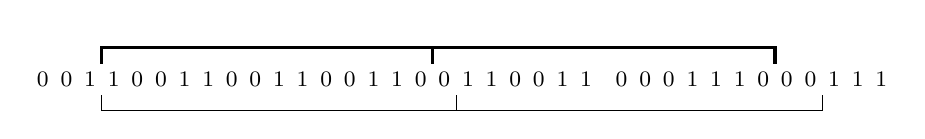
\begin{tikzpicture}[xscale=0.3]
  \foreach \x in {-11,-7,-3,1,5,9}{
    \begin{scope}[xshift=\x cm]
    \foreach \y in {0,1} \draw[xshift=\y cm] node {\footnotesize 0};
    \foreach \y in {0,1} \draw[xshift=2cm,xshift=\y cm] node {\footnotesize 1};
    \end{scope}
  }
  \begin{scope}[xshift=12.5cm]
  \foreach \x in {1,7}{
    \begin{scope}[xshift=\x cm]
    \foreach \y in {0,1,2} \draw[xshift=\y cm] node {\footnotesize 0};
    \foreach \y in {0,1,2} \draw[xshift=3cm,xshift=\y cm] node {\footnotesize 1};
    \end{scope}
  }
  \end{scope}
  
  \draw[very thick] (5.5,0.2) -- (5.5,0.4) node[above] {\footnotesize } -- (20,0.4) -- (20,0.2);
  \draw[very thick] (-8.5,0.2) -- (-8.5,0.4) -- (5.5,0.4);

  \draw (6.5,-0.2) -- (6.5,-0.4) -- (22,-0.4) -- (22,-0.2);
  \draw (-8.5,-0.2) -- (-8.5,-0.4) -- (6.5,-0.4);
\end{tikzpicture}
     \caption{
      Consider the word  and its subword .
      This subword corresponds to a balanced Abelian square with square vector
       (in bold).
      The first half of the Abelian square is followed with  and the second half with .
      Hence, if we extend each half by one position, we obtain an unbalanced Abelian square
      with square vector .
    }\label{fig:lb}
  \end{figure}

  
  An illustration of the proof of \cref{lem:balanced} is shown in \cref{fig:lb}.
  This figure also provides some intuition on how to obtain unbalanced Abelian squares
  from the balanced Abelian squares that we identified using this lemma.
  
  \begin{lemma}\label{lem:unbalanced}
  For each  the word  contains at least 
  square vectors of the form  for some integer .
  \end{lemma}
  \begin{proof}
  By \cref{lem:balanced}, there exists  whose square vector is .
  Moreover, it occurs in  at position .
  
  We shall prove that for each , 
  there is an Abelian square with square vector  occurring in  at position ; see also \cref{fig:unbalanced}.
  
  Note that  ends with  and is followed by ,
  while its first half ends with  (with  in particular) and is followed by 
  (by  in particular, because ). 
  Consequently, we have
  
  and
  
  Therefore, there are at least 
  square vectors of the claimed form in .  
  \end{proof}


  \begin{figure}[t]
    \centering
    \def\blockH{0.6}
\newcommand{\drawBlock}[4]{
  \draw[fill=white] (#1,0)--(#1/2+#2/2,0)--(#1/2+#2/2,\blockH)--(#1,\blockH)--cycle;
  \draw[fill=white!70!black] (#1/2+#2/2,0)--(#2,0)--(#2,\blockH)--(#1/2+#2/2,\blockH)--cycle;
  \node at (#1+#2/4-#1/4,\blockH) [above] {\small #3};
  \node at (#1/2+#2/2+#2/4-#1/4,\blockH) [above] {\small #4};
}
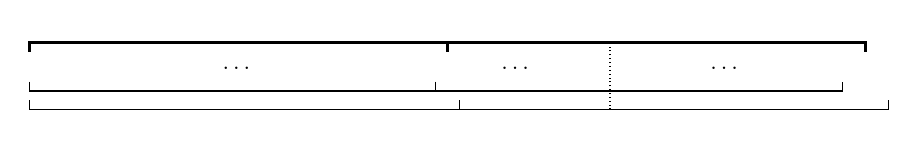
\begin{tikzpicture}[scale=0.295]

\drawBlock{-9}{-6}{}{}
\drawBlock{-6}{-3}{}{}
\drawBlock{-3}{0}{}{}
\drawBlock{4}{7}{}{}
\drawBlock{7}{10}{}{}
\drawBlock{10}{13}{}{}
\drawBlock{15}{18}{}{}
\drawBlock{18}{22}{}{}
\drawBlock{24}{28}{}{}
\drawBlock{28}{32}{}{}

\draw (2,0.3) node {\footnotesize \dots};
\draw (14,0.3) node {\footnotesize \dots};
\draw (23,0.3) node {\footnotesize \dots};

\draw[densely dotted] (18,-1.5) -- (18,1.5);

\draw[yshift=0.2cm,very thick,xshift=1cm] (10,0.8) -- (10,1.2) -- node[above=-2]{\scriptsize{}} (28,1.2) -- (28,0.8);
\draw[yshift=0.2cm,very thick,xshift=-17cm] (10,0.8) -- (10,1.2) -- node[above=-2]{\scriptsize{}} (28,1.2);

\draw[xshift=1cm] (-8,-0.3) -- (-8,-0.7) -- (9.5,-0.7);
\draw[xshift=18.5cm] (-8,-0.3) -- (-8,-0.7) -- (9.5,-0.7) -- (9.5,-0.3);

\
\draw[yshift=-0.8cm,xshift=1cm] (-8,-0.3) -- (-8,-0.7) -- node[below=-2]{\scriptsize{}} (10.5,-0.7);
\draw[yshift=-0.8cm,xshift=19.5cm] (-8,-0.3) -- (-8,-0.7) -- node[below=-2]{\scriptsize{}}  (10.5,-0.7) -- (10.5,-0.3);

\end{tikzpicture}
     \caption{\label{fig:unbalanced}
      A schematic illustration of the proof of \cref{lem:unbalanced}.
      Light rectangles represent zeroes and dark rectangles represent ones.
    }
  \end{figure}

  \begin{theorem}
     for each .
  \end{theorem}
  \begin{proof}
    We constructed a family of binary words  together with the sets .
    Note that 
    
    and, by \cref{obs:S},
    
    By \cref{lem:unbalanced}, the number of distinct square vectors in  is at least
    
    This completes the lower bound proof for .
    For other lengths  we pick the longest word  such that 
    and append it with ones.
  \end{proof}


  \section{Upper Bounds for Abelian Squares}\label{sec:upper}
  Let us start with an upper bound of  on the number
  of nonequivalent Abelian squares using the following result from additive combinatorics.
  Recall that an Abelian group  is called \emph{torsion-free} if  for  and  implies  or .
  \begin{lemma}[Katz \& Tao \cite{katz1999bounds}]\label{lem:tao}
  Let  be a torsion-free Abelian group, let  be subsets of , and let .
  If  then
  
  \end{lemma}

  \begin{observation}
    The set  (containing all Parikh vectors) with addition is
    a torsion-free Abelian group.
  \end{observation}
  
  \begin{theorem}
   for each  and .
  \end{theorem}
  \begin{proof}
  Consider a word  where  and a torsion-free Abelian group .
  For  let  be the Parikh
  vector of the -th prefix of . We set 
  
  and
  
  
  Note that  because every Abelian square has length at least 2.
  Moreover,  is an Abelian square if and only if ,
  so 
  This lets us use \cref{lem:tao} for  with .
  We obtain . However,
  since two Abelian squares  and  are equivalent if and only if ,
  we actually have 
  Since the choice of  was arbitrary, we conclude .
  \end{proof}
  
  \begin{remark}
    Katz \& Tao~\cite{katz1999bounds} apply a construction of Ruzsa \cite{ruzsa} to show
    that the upper bound on  cannot be improved beyond .
    However, their example does not seem to adapt to the setting of Abelian squares.
  \end{remark}
 
  In the second part of this section we show that a large number of
  Abelian squares enforces that a word contains a large number of blocks.
  Recall that a block is a maximal uniform fragment, i.e.,
  a maximal fragment whose letters are all equal.
  
  \begin{figure}[b]
 \centering
 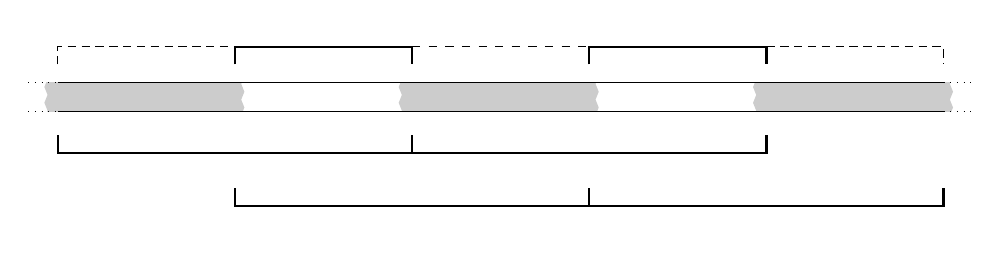
\begin{tikzpicture}[scale=0.75]


\begin{scope}
\clip (-1,0) rectangle (15,0.5);
\fill[decorate,decoration = {snake,amplitude =.2mm, segment length = 2mm},fill=black!20] (5.3,-1) rectangle (8.7,1);
\fill[decorate,decoration = {snake,amplitude =.2mm, segment length = 2mm},fill=black!20] (-.7,-1) rectangle (2.7,1);
\fill[decorate,decoration = {snake,amplitude =.2mm, segment length = 2mm},fill=black!20] (11.3,-1) rectangle (14.7,1);
\end{scope}
 \draw (4,0.25) node {};
 \draw (10,0.25) node {};
 \draw (-.5,0) -- (14.5,0) (-.5,.5) -- (14.5,.5);
 \draw[dotted] (-1,0) -- (-.5,0) (14.5,0) -- (15,0) (-1,.5) -- (-.5,.5) (14.5,.5) -- (15,.5);


  \draw[yshift=0.8cm,thick] (2.5,0) -- (2.5,0.3) -- (5.5,0.3) -- (5.5,0);
  \draw[xshift=3cm,yshift=0.8cm,dashed] (2.5,0.3) -- (5.5,0.3);
  \draw[xshift=6cm,yshift=0.8cm,thick] (2.5,0) -- (2.5,0.3) -- (5.5,0.3) -- (5.5,0);
  
  \draw (1,1.1) node[above] {\footnotesize{}};
  \draw (4,1.1) node[above] {\footnotesize{}};  
  \draw (7,1.1) node[above] {\footnotesize{}};
  \draw (10,1.1) node[above] {\footnotesize{}};  
  \draw (13,1.1) node[above] {\footnotesize{}};  


  \draw[densely dashed,yshift=0.8cm] (-0.5,0) -- (-0.5,0.3) -- (2.5,0.3);
  \draw[densely dashed,yshift=0.8cm,xshift=12cm] (-0.5,0.3) -- (2.5,0.3) -- (2.5,0);

  \begin{scope}[yshift=.6cm]
  \draw[yshift=-1cm,thick] (-0.5,0) -- (-0.5,-0.3) -- (5.5,-0.3) -- (5.5,0);
  \draw[xshift=6cm,yshift=-1cm,thick] (-0.5,-0.3) -- (5.5,-0.3) -- (5.5,0);
  \draw (5.5,-1.3) node[below] {\footnotesize{}};
\end{scope}
  \begin{scope}[xshift=3cm,yshift=-.3cm]
  \draw[yshift=-1cm,thick] (-0.5,0) -- (-0.5,-0.3) -- (5.5,-0.3) -- (5.5,0);
  \draw[xshift=6cm,yshift=-1cm,thick] (-0.5,-0.3) -- (5.5,-0.3) -- (5.5,0);
  \draw (5.5,-1.3) node[below] {\footnotesize{}};
  \end{scope}

\end{tikzpicture}
  \caption{
   Illustration of the ``'' case in the proof of \cref{lem:uniform}.
   Dark fragments represent occurrences of the same letter .
   In the proof we show that the dashed fragments all have the form , hence the two Abelian squares
   in the bottom have the same Parikh vectors.
 }\label{fig:uni}
\end{figure}

  \begin{lemma}\label{lem:uniform}
  Let  be a word,  be a positive integer and let , , be indices such that  and 
  are Abelian squares. If  is uniform, then .
  \end{lemma}
  \begin{proof}
  Let us define  so that .
  First, we suppose that . 
  In this case 
  
  and thus .
  
  Consequently, we may assume that ; see \cref{fig:uni}. As  and  are Abelian squares, we have
  
  Since  overlaps with  on , and  overlaps with  on 
  (see the upper part of \cref{fig:uni}), this yields:
  
  Hence, due to , we must also have  and .
  Because
  
  this concludes the proof.  
  \end{proof}
  
  \begin{theorem}\label{thm:ab-upper-bound-k-blocks}
    A word  of length  with  blocks contains at most  non\-equivalent Abelian squares of any fixed length. 
    Consequently, 
  \end{theorem}
  \begin{proof}
    Suppose that there are  nonequivalent Abelian squares of length .  
    Let us fix an arbitrary occurrence of each square and let  be their starting positions. 
    By \cref{lem:uniform}, none of the words , , is uniform. 
    Consequently,  has at least  blocks, i.e., .
  \end{proof}

  \cref{thm:ab-upper-bound-k-blocks} in particular implies a tight asymptotic bound for the
  number of non-equivalent Abelian squares in the lower-bound family of words .
  \begin{observation}
    .
  \end{observation}

  \section{Bounds for Order-Preserving Squares}\label{sec:op}
  Recall that  is an order-preserving square if  and there exists a strictly increasing
  bijection  such that  for all .

  \begin{remark}\label{rmk:op_last}
    A known property of ordinary squares is that each position of a word contains at most
    two rightmost occurrences of a square; see \cite{fraenkel-simpson}.
    This property immediately implies that a word of length  contains at most  distinct squares.
    Unfortunately, for order-preserving squares an analogous property does not hold.
    For example, the following word of length 28 being a permutation of :
    
    contains three rightmost occurrences of nonequivalent order-preserving squares (of lengths 16, 20, and 28) starting at the first position.
  \end{remark}
  
  Recall that  is a parameterized square
  if  and there is a bijection  such that
   for all .
  Note that, obviously, every order-preserving square is a parameterized square.
  A parameterized square  is called \emph{imbalanced} if .

  \begin{lemma}\label{lem:imbalanced}
  Let  and .
  At most  fragments of  are imbalanced parameterized squares.
  \end{lemma}
  \begin{proof}
    It suffices to prove that at most  prefixes of  are imbalanced parameterized squares.
  We shall construct an injective function  mapping such squares to 2-element subsets of :
  we define  where  is leftmost letter in  which does not belong to , and  is its counterpart in ,
  i.e.,  where  is the bijection corresponding to .
  Let  be the leftmost position such that  and .
  Observe that  and 
  are the leftmost occurrences of  and , respectively, in . Consequently,  can be reconstructed
  as the difference between these two positions. Hence,  is indeed an injection.
  \end{proof}
  
  \begin{corollary}\label{cor:op}
  Let  and . At most  fragments of 
  are order-preserving squares but not ordinary squares.
  \end{corollary}
  \begin{proof}
  Let  be an order-preserving square. If , then  is an imbalanced
  parameterized square. Otherwise, the corresponding monotone bijection  must be the identity.
  Hence,  is an ordinary square. Consequently, \cref{lem:imbalanced} concludes the proof.
  \end{proof}
  
  \begin{theorem}\label{thm:op}
  .
  \end{theorem}
  \begin{proof}
  A result of Deza et al.~\cite{DBLP:journals/dam/DezaFT15} shows that a word of length  contains
  at most  distinct ordinary squares.
  By \cref{cor:op}, the remaining order-preserving squares have at most  occurrences.
  \end{proof}

  
  \section{Bounds for Parameterized Squares}\label{sec:param}
  We start with a remark similar to \cref{rmk:op_last}.

  \begin{remark}
   The word
    
    contains three parameterized squares starting at the first position:
    
    such that no parameterized square equivalent to any of these three occurs anywhere else in the word.
  \end{remark}
  
  For a word  let us define  which results by removing all characters
  except for the \emph{last} occurrence of each letter. Note that in the resulting word
  each character of  occurs exactly once, i.e.,  is a \emph{permutation} of .
  We denote the family of permutations of  by .
  Throughout this section we consider permutations as strings over , i.e., .
  For a permutation  and a letter  we define  as the 0-based index of  in 
  \emph{counting from the right}. We extend  to arbitrary words  and characters  setting ,
  i.e.,  is the number of distinct characters after the last occurrence of  in .
  
  For a permutation  we define an encoding
   where  is a word  of length 
  such that for  we have .
  Intuitively,  shows, for each position  of , how many distinct letters are there between
   and the previous occurrence of the letter  in .
  However, if  occurs for the first time at position ,  uses the word 
  that is prepended to  to determine the previous occurrence.
  
\begin{example}
We have  and .
For  we have
; see Table~\ref{tab:1}. We also have .

\begin{table}[h]
  \begin{center}
    \caption{Intermediate steps of the computation of  for .}\label{tab:1}
    \footnotesize  
  \begin{tabular}{c|c|c|c|c}
     &  &  &  & \\\hline
      1 &  &  &  & 2 \\
      2 &  &  &  & 2 \\
      3 &  &  &  & 2 \\
      4 &  &  &  & 1 \\
      5 &  &  &  & 2 
  \end{tabular}
\end{center}
\end{table}
\end{example}

Below, we relate parameterized square prefixes of a word  with ordinary square prefixes of its encodings .
More precisely, we show that 
has a parameterized square prefix of a given length if and only if there exists a permutation  such that  has an (ordinary) square prefix of the same length. We start by listing a few simple properties of the notions introduced above.


\begin{observation}\label{obs:ord}
For every words  and every bijection  (extended to a morphism ), we
have
\begin{enumerate}[(i)]
  \item ,
  \item ,
  \item ,
  \item .
\end{enumerate}
\end{observation}

\begin{lemma}\label{lem:eq}
Let , , and .
If , then  and  are equivalent in the parameterized sense.
\end{lemma}
\begin{proof}
We proceed by induction on the length of the fragments. For length 0 the claim is trivial.
Thus, suppose that it holds for all lengths strictly smaller than . 
Consequently,  and  are parameterized equivalent with some witness bijection .

We consider two cases. First, suppose that

By definition of  this means that  and .
Consequently,  can be extended with , which yields the witness bijection for equivalence of 
and .

Next, suppose that

This means that  is the -th element of  ordered according to the last occurrence in .
Similarly,  is the -th element of  ordered in the same way with respect to .
Since  and  are parameterized equivalent, the relative positions of these last occurrences are the same.
Hence,  and  is the witness bijection of equivalence between  and .
\end{proof}

\begin{lemma}\label{lem:comp}
Let , , and let .
For every  we have .
\end{lemma}
\begin{proof}
Let us consider a position  of . If , we clearly have 

since . Thus, let us consider .
Then, we have

since  by \cref{obs:ord}(ii).
\end{proof}

\begin{lemma}\label{lem:pi}
Let  be a parameterized square. There exists  such that 
is an ordinary square. 
\end{lemma}
\begin{proof}
Let  be the decomposition into halves and let  be the witness bijection
of the parameterized equivalence of  and .
By \cref{lem:comp}, we have .
We shall choose  so that . 

Let us extend  to a bijection
 using identity on  and
an arbitrary bijection 
where  and .

Let  be the rank of , i.e., the smallest positive integer such that ,
and let  be an arbitrary permutation.
We claim that  is a permutation of  satisfying .
First, note that  and , so .
Next, we apply \cref{obs:ord}:

Finally, using \cref{obs:ord}(iv), we conclude that  since  and .
\end{proof}
 
 Next, we shall apply the following standard result to prove its counterpart for parameterized equivalence.
  \begin{fact}[\cite{fraenkel-simpson}]\label{fct:fraenkel}
  A word  has at most two prefixes which are ordinary squares without another occurrence in .
  \end{fact}
  
\begin{lemma}\label{lem:factorial}
A word  has at most  prefixes which are parameterized squares
without another (parameterized) occurrence in .
\end{lemma}
\begin{proof}
By \cref{lem:pi} for every prefix of  being a parameterized square there is a permutation 
such that the corresponding prefix of  is an ordinary square. Fact~\ref{fct:fraenkel} implies
that for a fixed  at most two such ordinary squares do not occur later in . However,
by \cref{lem:eq}, such a later occurrence in  means that the prefix of  has
another (parameterized) occurrence in . Combining these results yields an upper bound of 
on the number of prefixes being parameterized squares
without another (parameterized) occurrence in .
\end{proof}

\Cref{lem:factorial} immediately yields a bound for the parameterized squares.

\begin{theorem}
For every positive integers  and  we have 
     
    and .
\end{theorem} 
\begin{proof}
First, let us count parameterized squares up to equivalence.
\Cref{lem:factorial} implies that at most  parameterized squares have their leftmost occurrence
at any given position, which gives  non-equivalent parameterized squares in total.

To count parameterized squares up to equality of subwords, it suffices to observe that
every class of parameterized equivalence has at most  elements (the class  has exactly  elements).
Hence, the number of parameterized squares distinct as subwords is at most . 
\end{proof}


\section{Infinite Words Avoiding Nonstandard Squares and Cubes}\label{sec:infinite}
  Let us recall that there exist infinite ternary words that avoid ordinary squares \cite{Thue}
  (and obviously there is no such binary word).
  It is also known that there are infinite words over a 4-letter alphabet avoiding Abelian squares
  while over 3-letter alphabets such words do not exist \cite{DBLP:conf/icalp/Keranen92}.
  Here, we investigate an analogous problem for other nonstandard repetitions.

\subsection{Avoiding Order-Preserving Squares}
  We say that a word is op-square-free if it does not contain an order-preserving square
  of length greater than 2.
  Let  ordered in the natural way. Consider the morphism:
    
  It satisfies the following property, which lets us construct an op-square-free word. 

    \begin{observation}\label{obs:simple}
      For every symbols  we have:
      \begin{enumerate}[(i)]
        \item ;
        \item .
      \end{enumerate}
    \end{observation}

  \begin{lemma}\label{lem:left}
    If a word  is square-free, then  is op-square-free.
  \end{lemma}

  \begin{proof}
    Let  denote the order-preserving equivalence
    (i.e.,  if  and  is an order-preserving square).

    \noindent
    Suppose to the contrary that  contains an order-preserving square
    , with .
    We consider four cases depending on the parity of  and .

    If  and , then  and  start with a 1 and every second symbol of each of them is a 1.
    Consequently, by \cref{obs:simple}(i), .
    Moreover, in this case we have  and  for some subword  of .
    Hence,  is a square in , a contradiction.

    If  and , then  is also an order-preserving square.
    The conclusion follows from the previous case.

    If  and , then  and  start with  and  for some
    , respectively.
    By \cref{obs:simple}(ii), we conclude that , which implies a square  in , a contradiction.

    The final case,  and , also implies a 2-letter square in 
    just as in the previous case.
    This completes the proof that  is op-square-free.
  \end{proof}

  \noindent
  We apply \cref{lem:left} to all prefixes of an infinite square-free word \cite{Thue} over a ternary alphabet
  and obtain the following result.

  \begin{theorem}
    There exists an infinite op-square-free word over 3-letter alphabet.
  \end{theorem}

  \begin{example}
    If we apply the morphism  to the infinite square-free word that starts with
    \begin{center}
      012021012102012021\,
    \end{center}
    we obtain an op-square-free word that starts with:
    \begin{center}
      10\,11\,12\,10\,12\,11\,10\,11\,12\,11\,10\,12\,10\,11\,12\,10\,12\,11\,
    \end{center}
  \end{example}
  
  
\subsection{Avoiding Parameterized Cubes}
  A parameterized cube is a word  such that both  and  are parameterized squares.
  A word is called parameterized-square-free (parameterized-cube-free)
  if it does not contain parameterized squares (parameterized cubes) of length
  greater than 3.
  We show that there is no infinite parameterized-square-free word,
  and we construct a binary parameterized-cube-free word.

  \begin{theorem}
    There is no infinite parameterized-square-free word.
  \end{theorem}
  \begin{proof}
    Suppose to the contrary that such an infinite word  exists.
    In the proof we denote symbols of  by .
    Note that every suffix of  has to contain two adjacent equal symbols.
    This is because  for  and  is a parameterized square.
    Moreover,  has to contain some three adjacent equal symbols.
    The reason is that  for  is a parameterized square.

    We can therefore assume that  contains a subword .
    To avoid a parameterized square of length 4, this subword must be followed in 
    by some letter .
    For the same reason the next letter  must satisfy , and afterwards
    the subword  must be followed by two more occurrences of .
    Finally the next letter must be  to avoid a parameterized square .
    We conclude that  contains a subword  for  and ,
    which turns out to be a parameterized square.
    This contradiction completes the proof.
  \end{proof}

  We proceed to a construction of a binary parameterized-cube-free word.
  An \emph{antisquare} is a nonempty word of the form , where  denotes bitwise negation of .
  For example, 011 100 is an antisquare.
  In the proof we will use the following characterisation of binary parameterized squares.
  
  \begin{observation}\label{obs:anti}
    For binary alphabet each parameterized square is an ordinary square or an antisquare.
  \end{observation}

  Let  be the infinite Thue-Morse word.
  Recall that  is cube-free \cite{Thue2}.
  Also recall the morphism  defined just before \cref{lem:left}
  (here we consider only  and ).

  \begin{theorem}
    The word  is parameterized-cube-free.
  \end{theorem}
  \begin{proof}
    Suppose to the contrary that  is a parameterized cube in , with
    .
    Note that  does not contain 6 ones in a row.
    Hence, at least one of the words  contains 0, therefore each of them contains 0.
    Moreover, every second symbol of  is 1.

    Recall from \cref{obs:anti} that a binary parameterized square is either
    an ordinary square or an antisquare.
    If , then the ones of every second position of  align
    and ,  must be ordinary squares.
    Therefore  is an ordinary cube in  which induces a cube in .

    If , the same argument implies that both  and  are antisquares.
    Because of the ones on every second position of 
    we actually have , ,  or
    , , .
    In both cases we obtain a cube  in  which induces   in .
  \end{proof}

  \begin{example}
    The first few symbols of the Thue-Morse word  are:
    \begin{center}
      011010011001011010\,
    \end{center}
    We apply the morphism  to obtain a parameterized-cube-free word
    starting with:
    \begin{center}
      10\,11\,11\,10\,11\,10\,10\,11\,11\,10\,10\,11\,10\,11\,11\,10\,11\,10\,
    \end{center}
  \end{example}

  \section{Final Remarks}
  We have presented several combinatorial results related to the maximum number of
  nonstandard squares in a word of length .
  For Abelian squares we have shown that for :
  

  For squares in order-preserving and parameterized setting we have shown
  that their maximum number is linear of  for a constant alphabet.
  We have also presented examples of infinite words over a minimal alphabet that avoid squares in
  order-preserving setting and cubes in parameterized setting, respectively.

  The main open question that arises from our work is to provide an upper bound for .
  We have made a step towards this bound by showing that the maximum number of distinct Abelian squares
  in a word of length  containing  blocks is .
  The remaining open questions are connected to  and 
  for arbitrary  (not necessarily a constant).
  Based on experimental results, we state the following hypothesis:
\begin{hypothesis}
   For every ,
  , , and 
  (with constant factors independent of ).
\end{hypothesis}

\begin{comment}
  A tempting idea effectively used for ordinary squares would be to consider only the \emph{last occurrence}
  of each type of Abelian square and show that the maximum number of such occurrences starting at the same position
  of the word (or sharing the same middle interposition) is small.
  Unfortunately, this number can be large, e.g.,
  the word  of length  contains  different square vectors ,
  each corresponding to a last occurrence of Abelian square at the first position,
  whereas the word  also of length , contains last occurrences of  different
  Abelian squares centered at its center.
  Another idea could be to try to bound the maximum number of nonequivalent (long) Abelian squares in a word of the same length.
  However, this number also can be large, e.g.\ the word  of length 
  contains  nonequivalent Abelian squares of length  (namely, , , \ldots, ).
\end{comment}


\bibliographystyle{plainurl}
\bibliography{squares}


\end{document}
